\documentclass{article}
\usepackage[T1]{fontenc}
\usepackage{lmodern}
\usepackage{graphicx}
\usepackage{amsmath,amssymb}
\usepackage[a4paper,margin=2cm]{geometry}
\usepackage[absolute,overlay]{textpos}
\setlength{\TPHorizModule}{1mm}
\setlength{\TPVertModule}{1mm}
\usepackage[indonesian]{babel}
\usepackage{hyperref}
\setlength{\emergencystretch}{2em}
% unit: Halaman 21

\begin{document}

% === Halaman 21 (llm) ===

\begin{itemize}
    \item Dugaan kebocoran data pemilih Pemilu 2014, kebocoran sertifikat vaksin Jokowi
\end{itemize}

\vspace{10mm}

% deskripsi: Tangkapan layar berita Kompas.com mengenai kebocoran sertifikat vaksin Jokowi.
% bbox normalisasi: [0.1200, 0.2700, 0.5700, 0.9500]
\begin{textblock*}{94.50mm}(25.20mm,80.19mm)
\noindent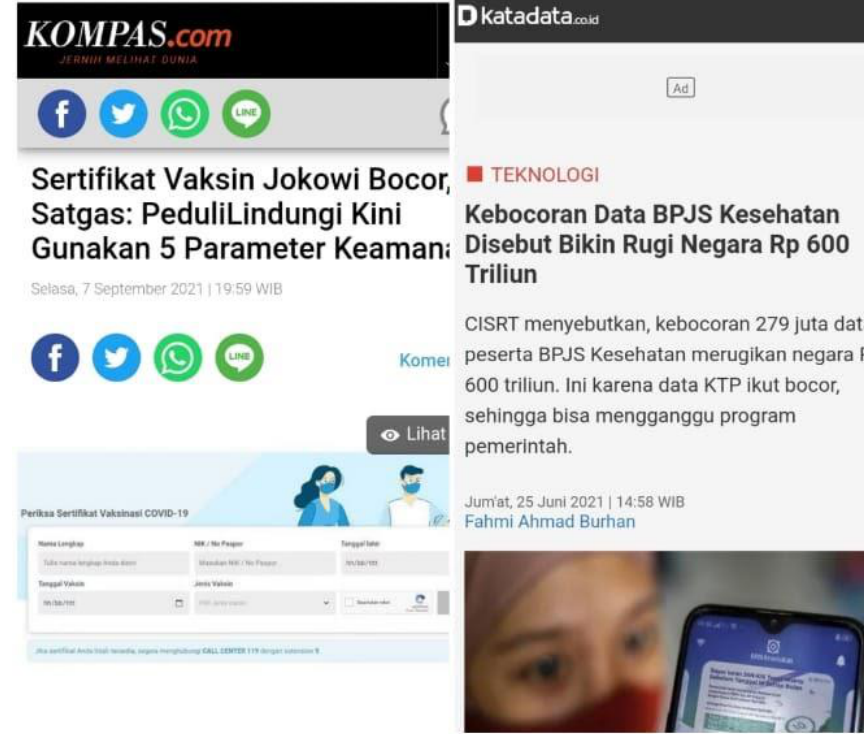
\includegraphics[width=94.50mm,height=201.96mm]{../../images/llm/page_021_img_01.png}%
\end{textblock*}

% deskripsi: Tangkapan layar berita Katadata mengenai kebocoran data BPJS Kesehatan.
% bbox normalisasi: [0.3500, 0.2600, 0.5800, 0.9500]
\begin{textblock*}{48.30mm}(73.50mm,77.22mm)
\noindent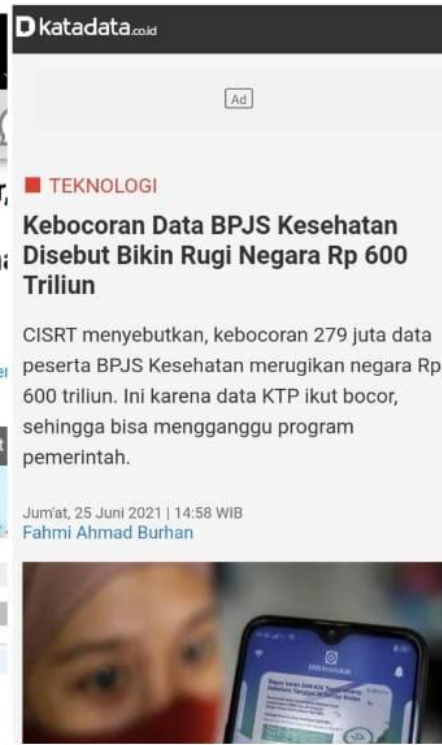
\includegraphics[width=48.30mm,height=204.93mm]{../../images/llm/page_021_img_02.png}%
\end{textblock*}

% deskripsi: Tangkapan layar berita Kompas.com mengenai dugaan kebocoran data pemilih Pemilu 2014.
% bbox normalisasi: [0.5800, 0.2600, 0.8200, 0.9500]
\begin{textblock*}{50.40mm}(121.80mm,77.22mm)
\noindent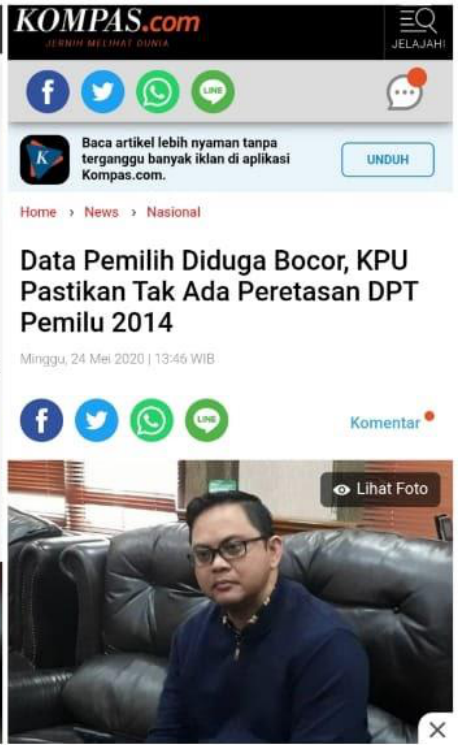
\includegraphics[width=50.40mm,height=204.93mm]{../../images/llm/page_021_img_03.png}%
\end{textblock*}

\end{document}
